\documentclass[11pt,a4paper]{article}
\usepackage[utf8]{inputenc}
\usepackage[spanish]{babel}
\usepackage{amsmath}
\usepackage{amsfonts}
\usepackage{amssymb}
\usepackage{graphicx}
\usepackage{enumitem}
\usepackage{geometry}
\usepackage{float}

\geometry{left=2.5cm,right=2.5cm,top=2.5cm,bottom=2.5cm}

\begin{document}

% --- ENCABEZADO ---
\begin{center}
    \textbf{UNIVERSIDAD TECNOLÓGICA NACIONAL \\ FACULTAD REGIONAL LA PLATA} \\
    \vspace{0.2cm}
    \textbf{INGENIERÍA MECANICA — Curso 2026} \\
    \vspace{0.2cm}
    \textit{Asignatura: ESTABILIDAD 1}
\end{center}

\vspace{0.3cm}

\begin{flushleft}
    \textbf{Prof. Titular:} Ing. Augusto Vaello \\
    \textbf{JTP:} Ing. Jorge Ronconi \\
\end{flushleft}

\noindent\rule{\linewidth}{0.4pt}

\begin{center}
    \vspace{0.4cm}
    \Large \textbf{Trabajo Práctico N°2: FUERZAS NO CONCURRENTES EN EL PLANO} \\
    \vspace{0.4cm}
\end{center}

% --- EJERCICIO 1 ---
\subsection*{Ejercicio N°1: Resultante de un sistema no concurrente}

Dado el sistema de fuerzas no concurrentes en el plano indicado en la Figura~1,
donde las fuerzas tienen los siguientes datos:

\begin{center}
\begin{tabular}{cccc}
\hline
\textbf{Fuerza} & \textbf{Módulo} & \textbf{Dirección} & \textbf{Punto de aplicación} \\
\hline
$F_1$ & 10 kN & $60^\circ$  & $( 3,\; 2)$ m \\
$F_2$ & 8 kN  & $270^\circ$ & $( 1,\; 0)$ m \\
$F_3$ & 6 kN  & $180^\circ$ & $( 0,\;-4)$ m \\
$F_4$ & 9 kN  & $225^\circ$ & $(-3,\; 1)$ m \\
\hline
\end{tabular}
\end{center}

\begin{enumerate}[label=\alph*)]
    \item \textbf{Analíticamente:} Determinar módulo, dirección y recta de acción
    de la resultante mediante dos ecuaciones de proyección y una de momentos
    respecto al origen.
    \item \textbf{Gráficamente:} Verificar mediante el método del polígono funicular,
    construyendo el polígono de fuerzas y localizando la recta de acción de la
    resultante.
\end{enumerate}

\begin{figure}[H]
    \centering
    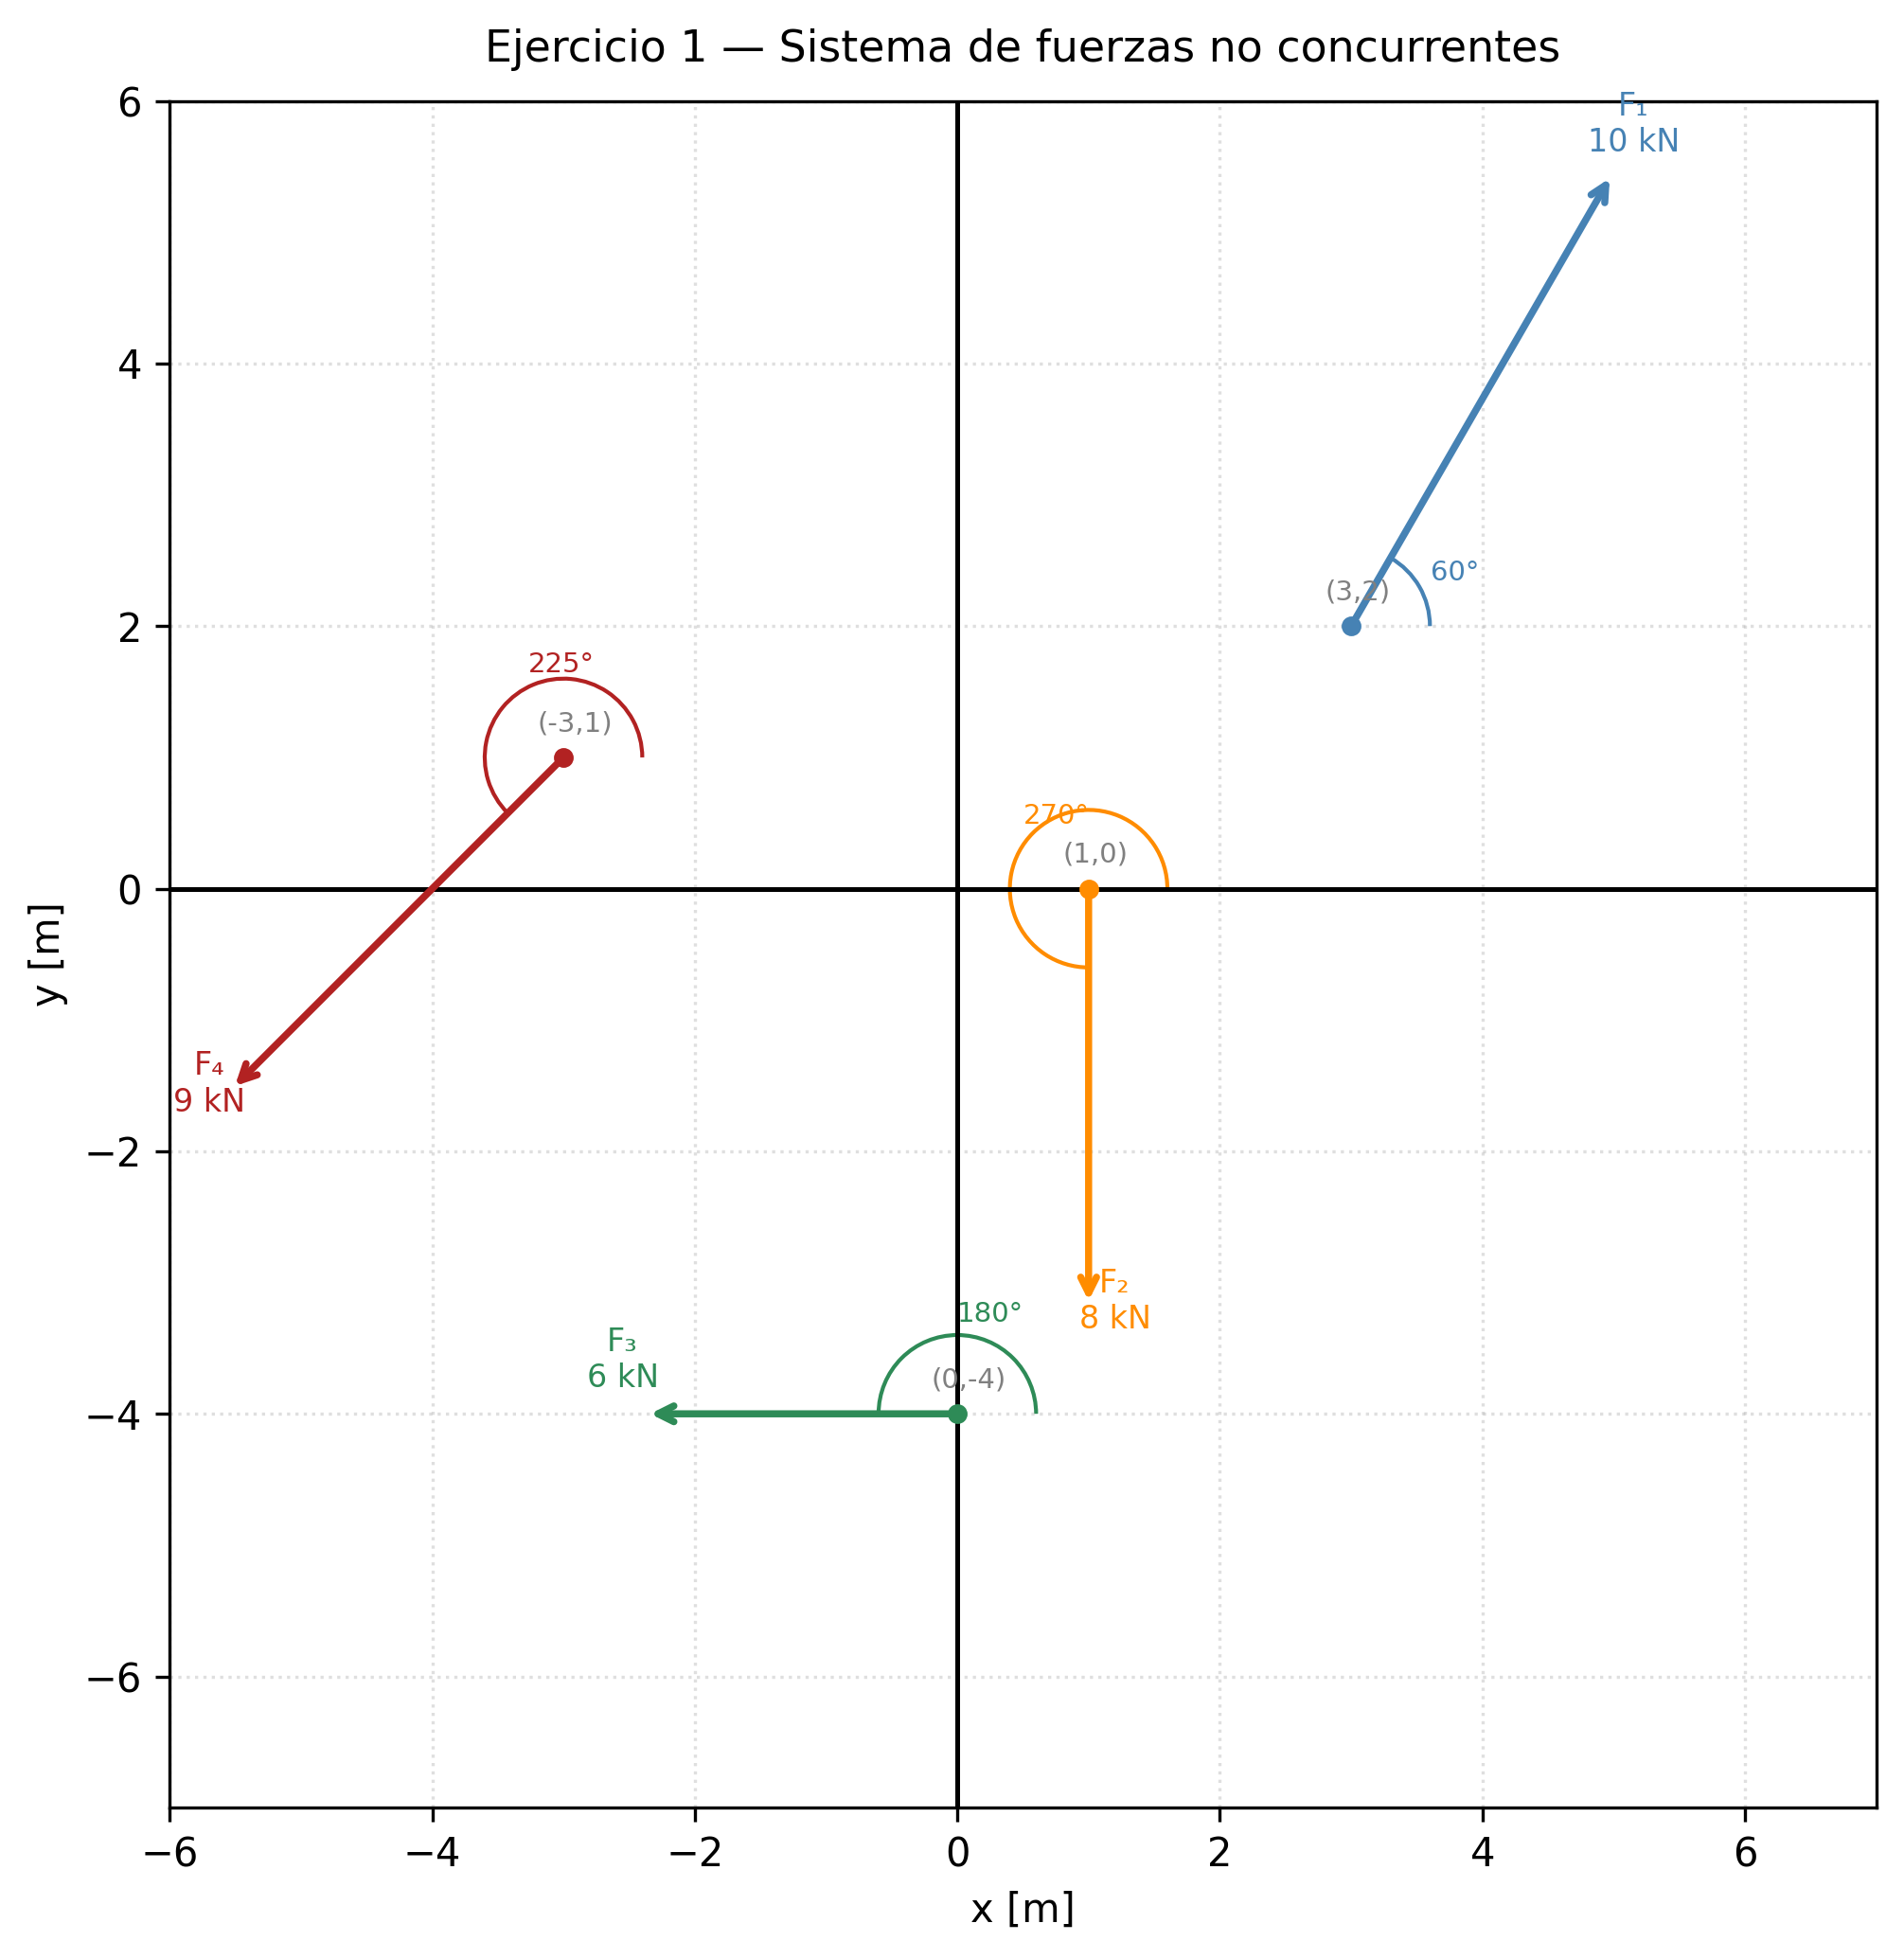
\includegraphics[width=0.60\textwidth]{img/tp/tp2_ej1.png}
    \caption{Sistema de fuerzas no concurrentes — Ejercicio 1.}
    \label{fig:ej1}
\end{figure}

% --- EJERCICIO 2 ---
\subsection*{Ejercicio N°2: Descomposición — Cullman y tres momentos}

Dada la fuerza $P = 12\,\text{kN}$ aplicada a $40^\circ$ respecto a la horizontal,
descomponerla en las tres direcciones no concurrentes $a$, $b$ y $c$ indicadas
en la Figura~2, mediante:

\begin{enumerate}[label=\alph*)]
    \item \textbf{Método de Cullman} (gráfico).
    \item \textbf{Método analítico:} tres ecuaciones de momentos.
\end{enumerate}

Las rectas de acción tienen los siguientes datos:

\begin{center}
\begin{tabular}{ccc}
\hline
\textbf{Dirección} & \textbf{Ángulo} & \textbf{Punto de paso} \\
\hline
$a$ & $55^\circ$ & $(0,\; 2)$ m \\
$b$ & $0^\circ$ & $(0,\; -2)$ m \\
$c$ & $270^\circ$ & $(2,\;0)$ m \\
\hline
\end{tabular}
\end{center}

\begin{figure}[H]
    \centering
    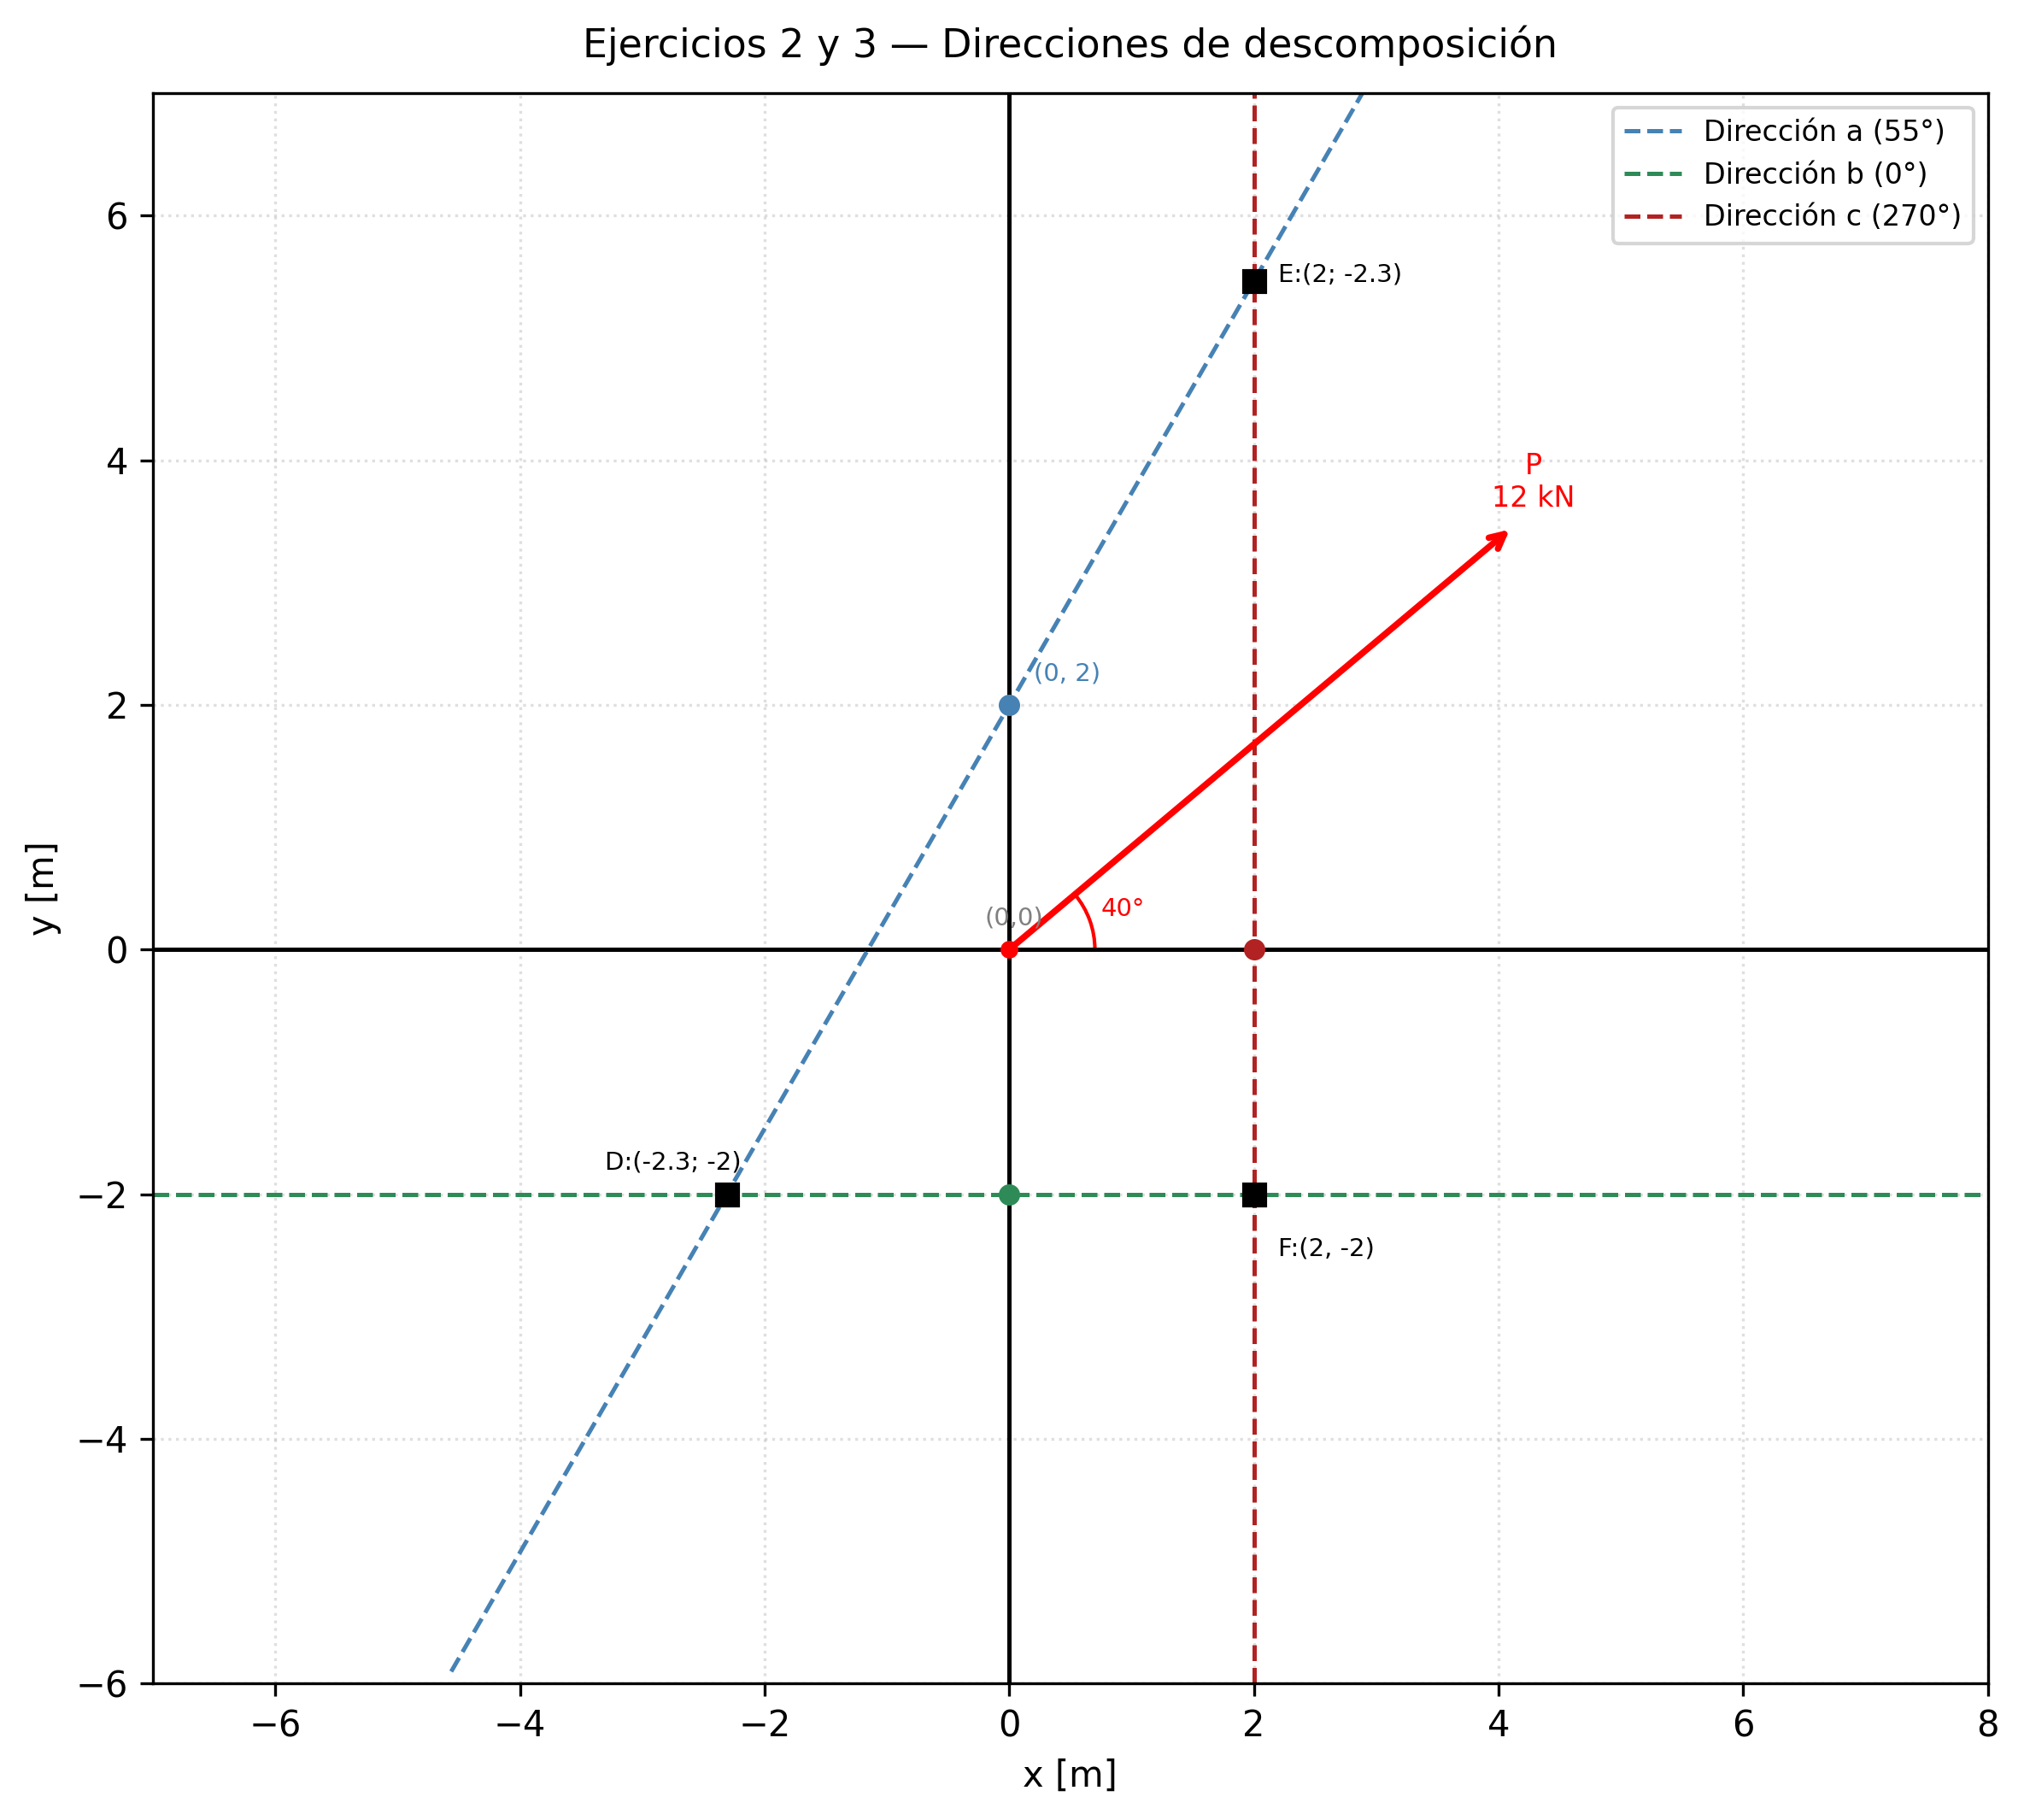
\includegraphics[width=0.70\textwidth]{img/tp/tp2_ej2.png}
    \caption{Direcciones de descomposición — Ejercicio 2.}
    \label{fig:ej2}
\end{figure}

% --- EJERCICIO 3 ---
\subsection*{Ejercicio N°3: Descomposición — proyecciones y Ritter}

Para el mismo sistema de la Figura~2, descomponer $P = 12\,\text{kN}$ a $40^\circ$
en las tres mismas direcciones $a$, $b$ y $c$, mediante:

\begin{enumerate}[label=\alph*)]
    \item \textbf{Método analítico:} dos ecuaciones de proyección y una de momentos.
    \item \textbf{Método de Ritter:} tres ecuaciones de momentos tomados en los puntos de intersección de las rectas de acción de a pares.
\end{enumerate}

Verificar que los resultados coincidan con los del Ejercicio~2.

% --- EJERCICIO 4 ---
\subsection*{Ejercicio N°4: Resultante con fuerzas paralelas}

Dado el sistema de fuerzas paralelas verticales indicado en la Figura~3:

\begin{center}
\begin{tabular}{ccc}
\hline
\textbf{Fuerza} & \textbf{Módulo} & \textbf{Punto de aplicación} \\
\hline
$F_1$ & 6 kN (↑) & $x = -3$ m \\
$F_2$ & 10 kN (↓) & $x = 0$ m \\
$F_3$ & 4 kN (↑) & $x = 2$ m \\
$F_4$ & 7 kN (↓) & $x = 5$ m \\
\hline
\end{tabular}
\end{center}

\begin{enumerate}[label=\alph*)]
    \item \textbf{Analíticamente:} Determinar la resultante y su punto de aplicación sobre el eje X mediante una ecuación de momentos respecto al origen.
    \item \textbf{Gráficamente:} Verificar con el polígono funicular.
    \item \textbf{Discusión:} ¿Qué ocurre si $\sum F_y = 0$ pero $\sum M \neq 0$? Identificar qué tipo de sistema resulta en ese caso.
\end{enumerate}

\begin{figure}[H]
    \centering
    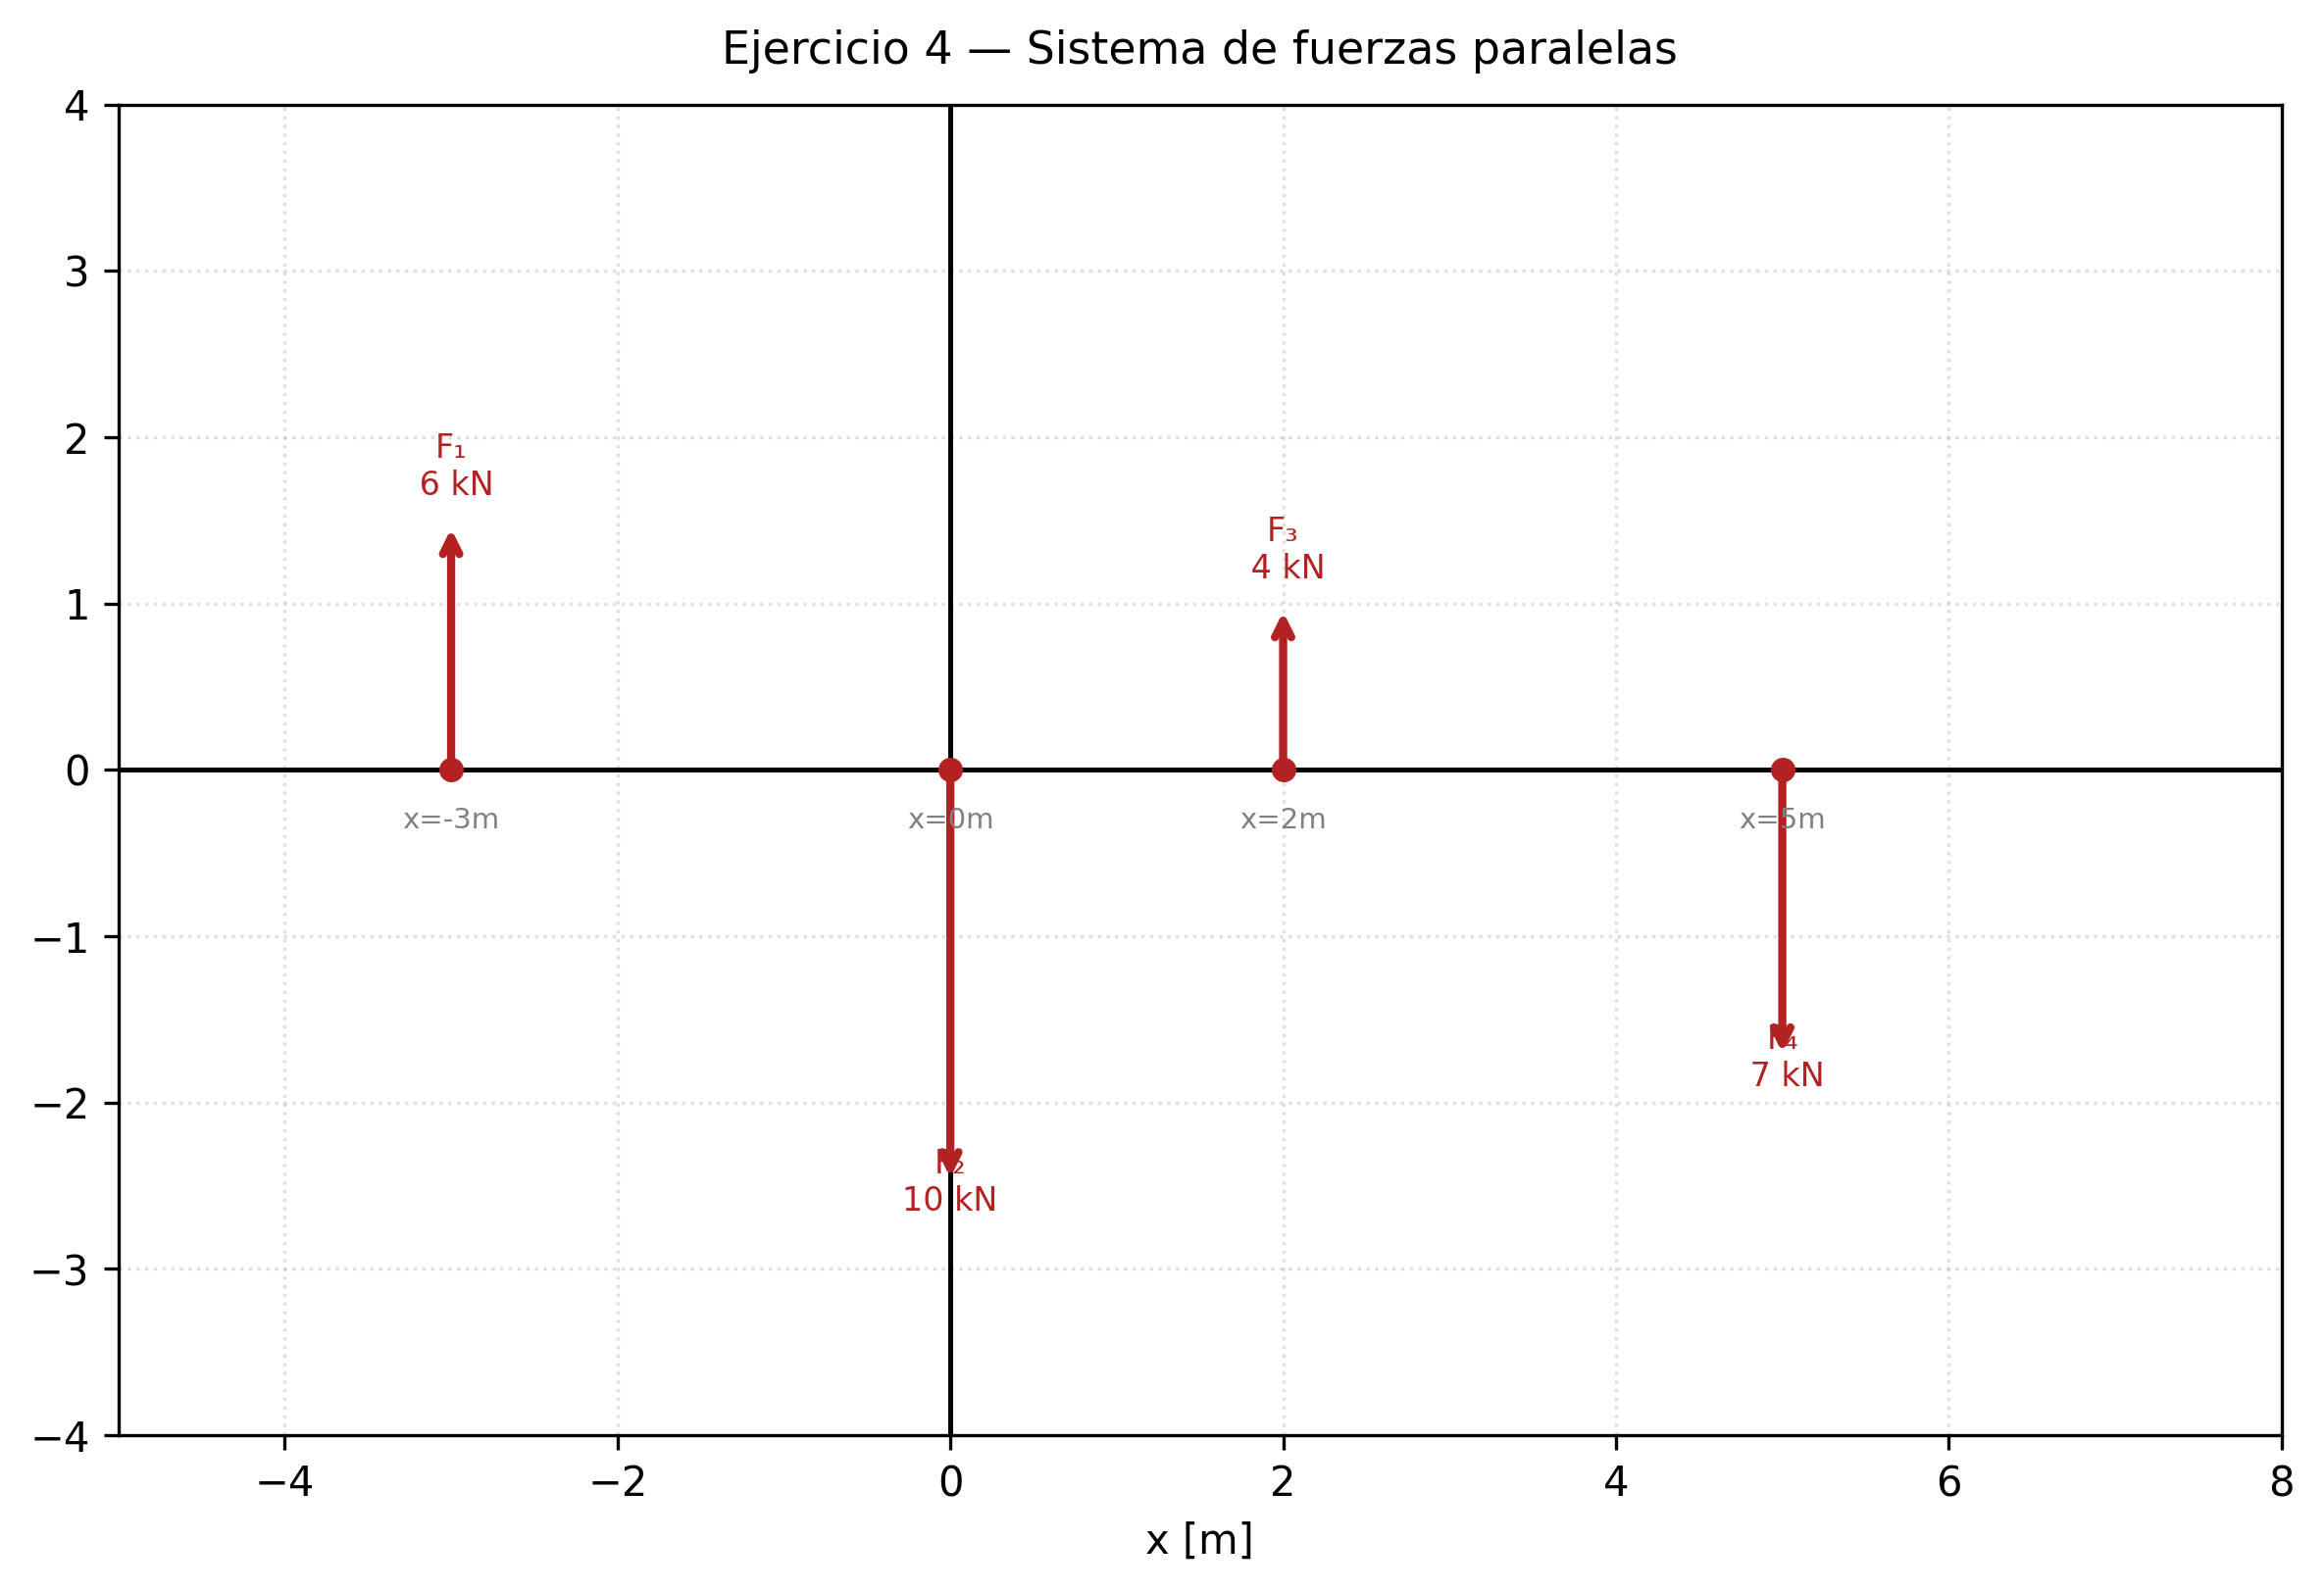
\includegraphics[width=0.65\textwidth]{img/tp/tp2_ej4.png}
    \caption{Sistema de fuerzas paralelas — Ejercicio 4.}
    \label{fig:ej4}
\end{figure}

% --- EJERCICIO 5 ---
\subsection*{Ejercicio N°5: Sistema con cupla resultante}

Dado el sistema de fuerzas no concurrentes de la Figura~5:

\begin{center}
\begin{tabular}{cccc}
\hline
\textbf{Fuerza} & \textbf{Módulo} & \textbf{Dirección} & \textbf{Punto de aplicación} \\
\hline
$F_1$ & 8 kN & $90^\circ$ (↑) & $(-2,\; 0)$ m \\
$F_2$ & 8 kN & $270^\circ$ (↓) & $(3,\; 0)$ m \\
$F_3$ & 5 kN & $0^\circ$ (→) & $(0,\; 2)$ m \\
$F_4$ & 5 kN & $180^\circ$ (←) & $(0,\;-2)$ m \\
\hline
\end{tabular}
\end{center}

\begin{enumerate}[label=\alph*)]
    \item \textbf{Analíticamente:} Calcular $R_x$, $R_y$ y el momento resultante
    $M_R$ respecto al origen. Identificar qué tipo de sistema resulta y expresar
    la equivalencia mecánica completa.
    \item \textbf{Gráficamente:} Construir el polígono de fuerzas y el polígono
    funicular. Observar qué ocurre con el funicular e interpretar geométricamente
    el resultado.
    \item \textbf{Discusión:} Explicar por qué este sistema no puede reducirse a
    una fuerza única y cómo se representa la cupla equivalente.
\end{enumerate}

\begin{figure}[H]
    \centering
    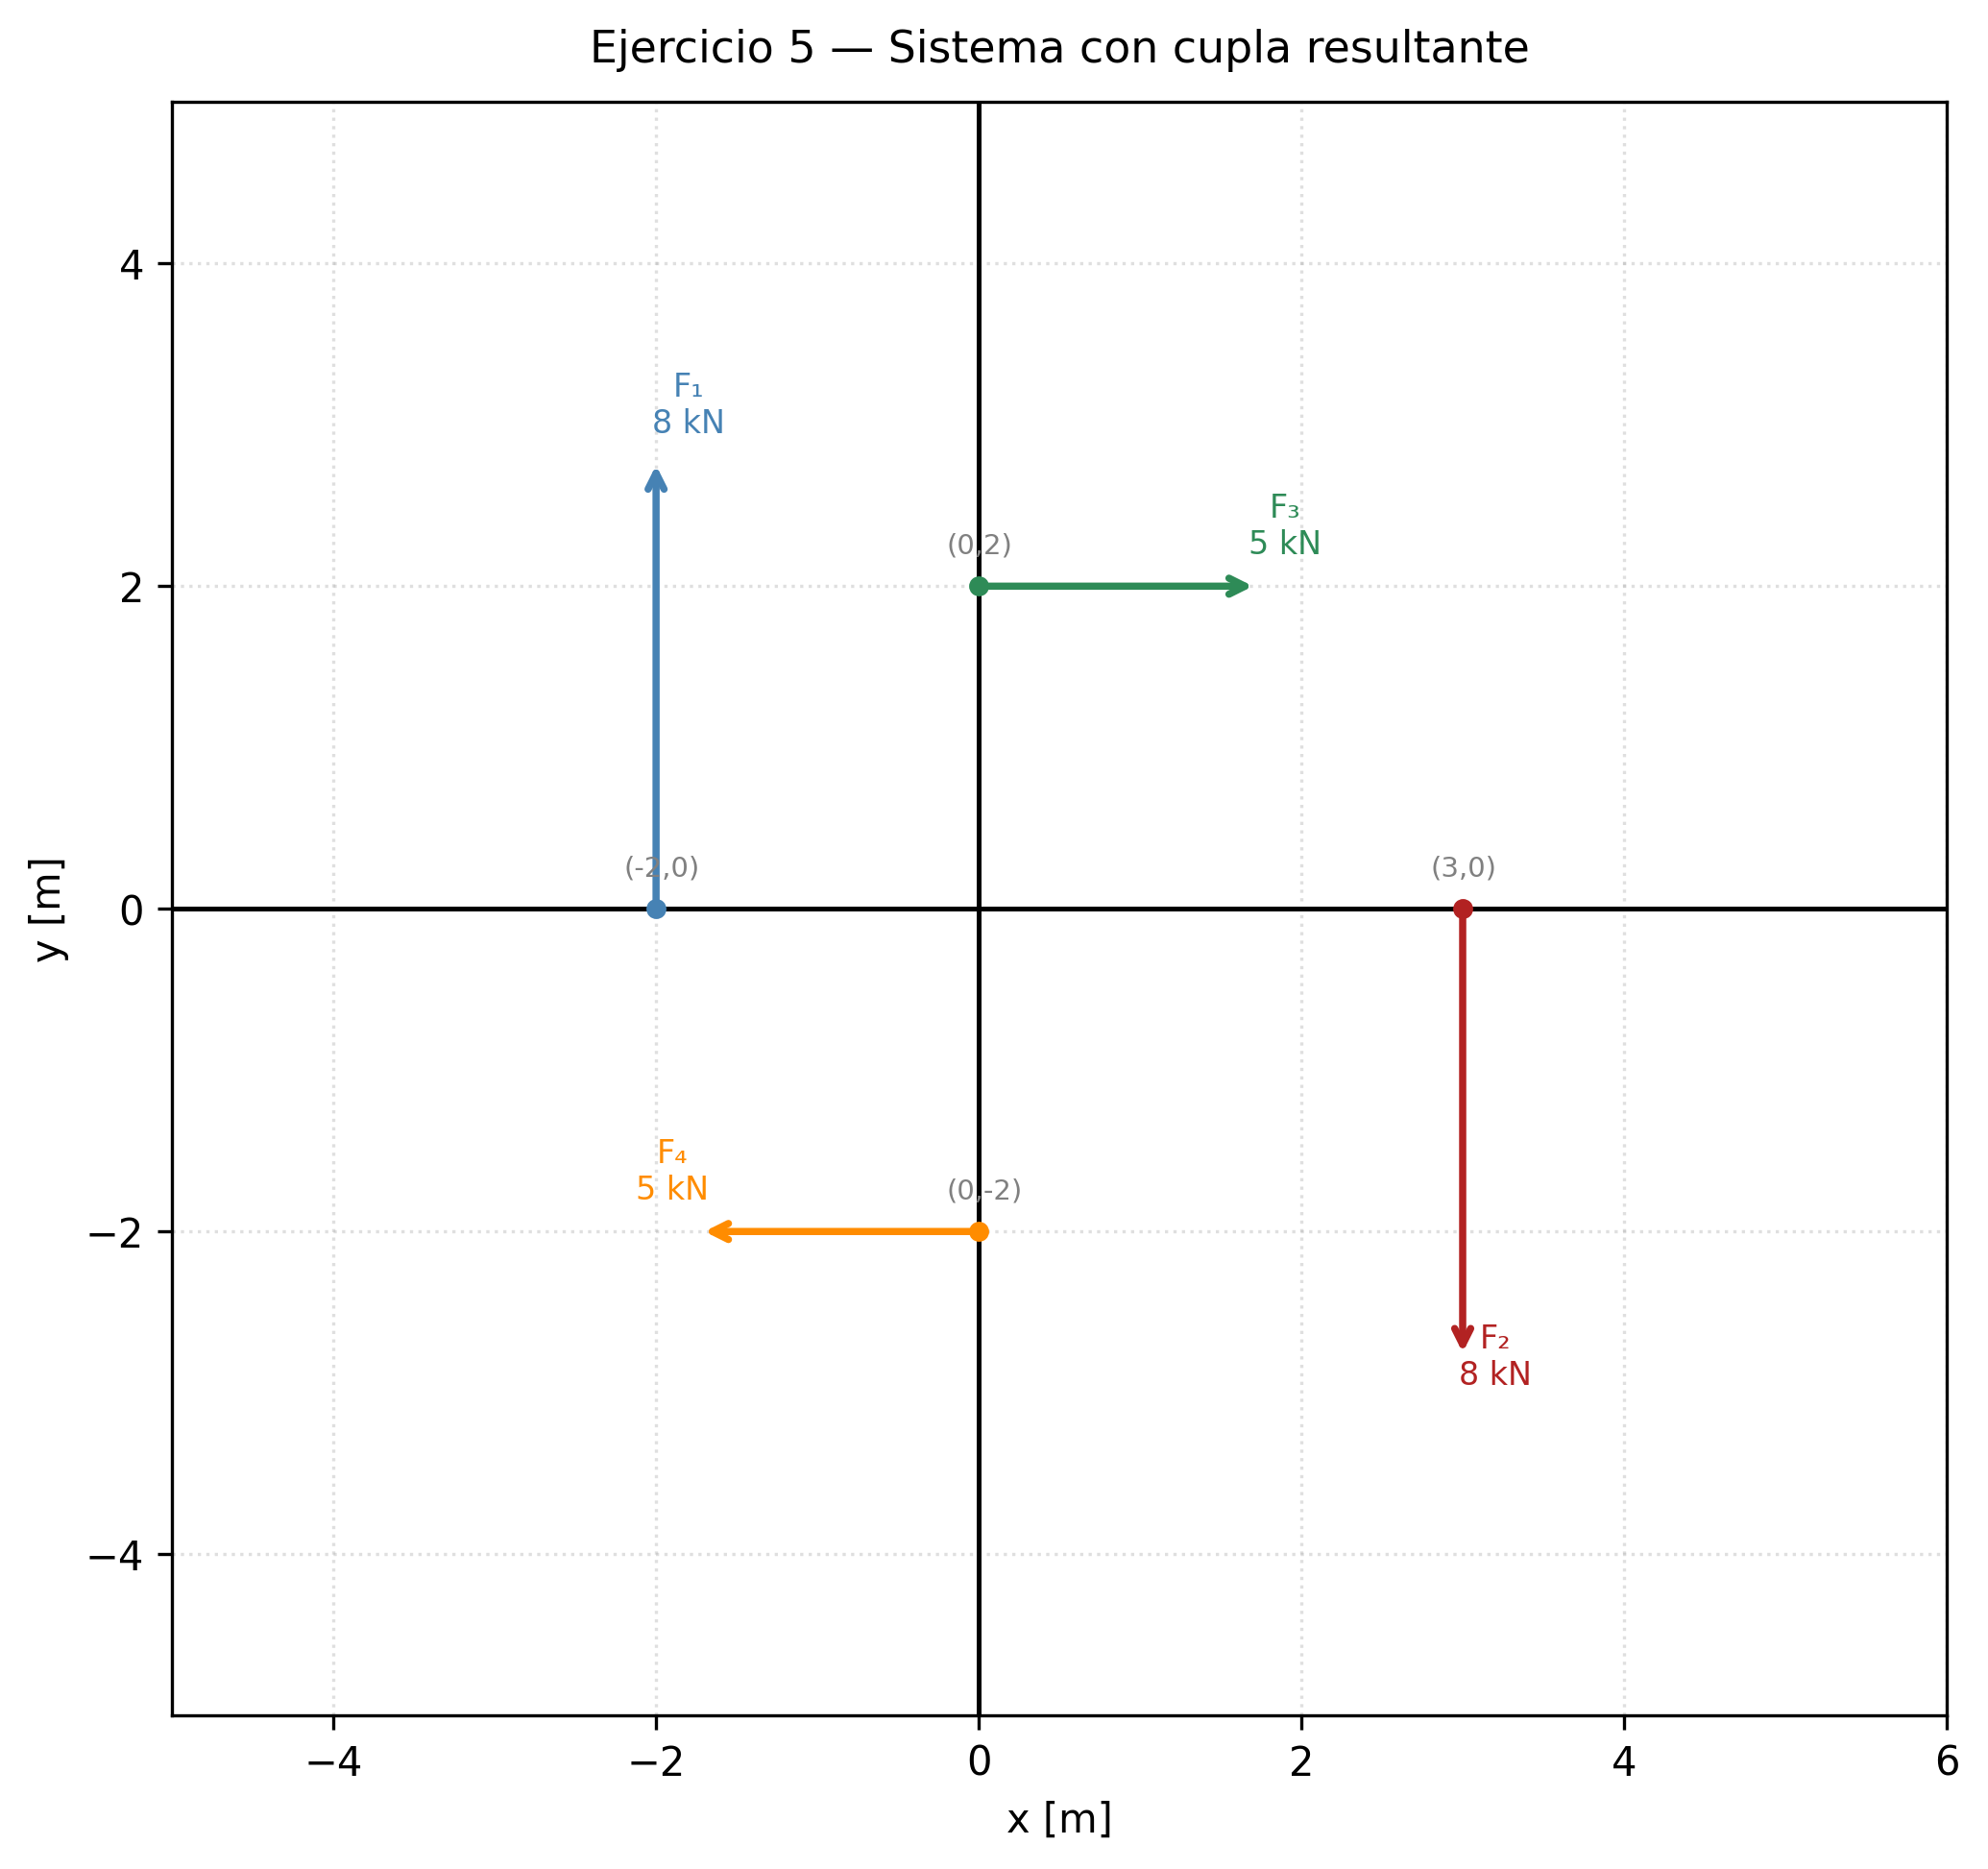
\includegraphics[width=0.65\textwidth]{img/tp/tp2_ej5.png}
    \caption{Sistema con cupla resultante — Ejercicio 5.}
    \label{fig:ej5}
\end{figure}

\end{document}